\section{Temporal Extent}
\label{sec:Temporal}
%%%%%%%%%%%%%%%%%%%%%%%%%%%%%%%%%%%%%%%%%%%%%%%%%%%%%%%%
\begin{figure}[h!]
\begin{center}
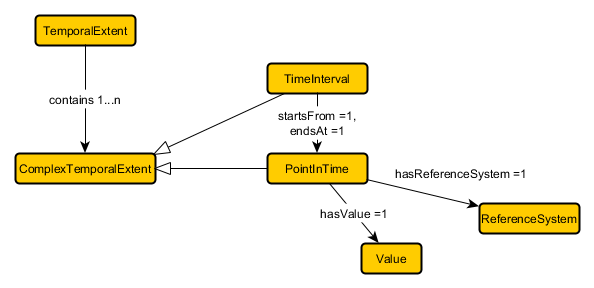
\includegraphics[width=.8\textwidth]{figures/temporal}
\end{center}
\caption{Schema Diagram for Temporal Extent. The visual notation is explained in Chapter \ref{chap:prelims}.}
\label{fig:Temporal}
\end{figure}
\subsection{Summary}
\label{sum:Temporal}
%%%%%%%%%%%%%%%%%%%%%%%%%%%%
I am some summary text.

%%%%%%%%%%%%%%%%%%%%%%%%%%%%%%%%%%%%%%%%%%%%%%%%%%%%%%%%
\subsection{Axiomatization}
\label{axs:Temporal}
%%%%%%%%%%%%%%%%%%%%%%%%%%%%
\begin{align}
\textsf{TemporalExtent} &\sqsubset \mathord{=}n \textsf{contains.ComplexTemporalExtent} \\
\textsf{TimeInterval} &\sqsubset \textsf{ComplexTemporalExtent} \\
\textsf{TimeInterval} &\sqsubset \mathord{=}1 \textsf{startsFrom.PointInTime} \\
\textsf{TimeInterval} &\sqsubset \mathord{=}1 \textsf{endsAt.PointInTime} \\
\textsf{PointInTime} &\sqsubset \textsf{ComplexTemporalExtent} \\
\textsf{PointInTime} &\sqsubset \mathord{=}1 \textsf{hasReferenceSystem.ReferenceSystem} \\
\textsf{PointInTime} &\sqsubset \mathord{=}1 \textsf{hasValue.Value}
\end{align}

%%%%%%%%%%%%%%%%%%%%%%%%%%%%%%%%%%%%%%%%%%%%%%%%%%%%%%%%
\subsection{Explanations}
\label{exp:Temporal}
%%%%%%%%%%%%%%%%%%%%%%%%%%%%
\begin{enumerate}
\item Numerical Restriction: a \textsf{TemporalExtent} \textsf{contains} exactly $n$ \textsf{ComplexTemporalExtents}. See below remarks.
\item Subclass: every \textsf{TimeInterval} is a \textsf{ComplexTemporalExtent}.
\item Numerical Restriction: a \textsf{TimeInterval} \textsf{startsAt} exactly 1 \textsf{PointInTime}.
\item Numerical Restriction: a \textsf{TimeInterval} \textsf{endsAt} exactly 1 \textsf{PointInTime}.
\item Subclass: every \textsf{PointInTime} is a \textsf{ComplexTemporalExtent}.
\item Numerical Restriction: a \textsf{PointInTime} has exactly 1 \textsf{ReferenceSystem}.
\item Numerical Restriction: a \textsf{PointInTime} has exactly 1 \textsf{Value}.
\end{enumerate}

%%%%%%%%%%%%%%%%%%%%%%%%%%%%%%%%%%%%%%%%%%%%%%%%%%%%%%%%
\subsection{Competency Question}
\label{cqs:Temporal}
%%%%%%%%%%%%%%%%%%%%%%%%%%%%
\begin{enumerate}[CQ1.]
\item How long was World War II?
\item What era was the ice age?
\end{enumerate}

\newpage
%%%%%%%%%%%%%%%%%%%%%%%%%%%%%%%%%%%%%%%%%%%%%%%%%%%%%%%%
% End Section
%%%%%%%%%%%%%%%%%%%%%%%%%%%%%%%%%%%%%%%%%%%%%%%%%%%%%%%%
%%%%%%%%%%%%%%%%%%%%%%%%%%%%%%%%%%%%%%%%%%%%%%%%%%%%%%%%